\begin{sectionbox}{ucblue}{CASOS CHILENOS (2021-2025)}

\subsection*{\textcolor{ucred}{\textbf{2021: Bots y Segmentación Generacional}}}
{\fontsize{20}{24}\selectfont
\textbf{Plataformas:} TikTok (generacional), WhatsApp (cerrada)

\textbf{Mecanismo:} 20,000 bots crean consenso falso.

\textbf{Casos Reales:}
\begin{itemize}
    \item \textbf{Evelyn Matthei:} Narrativa falsa sobre Alzheimer.
    \item \textbf{Elisa Loncón:} Fotomontajes con Pinochet.
\end{itemize}

\textbf{Resultado:} Debate polarizado sin diálogo transversal
}

\vspace{0.2cm}

\subsection*{\textcolor{ucred}{\textbf{2022-2023: Plebiscito Manipulado}}}
{\fontsize{20}{24}\selectfont
\textbf{1 abril 2022 (Inflexión CADEM):} Titular de Fontaine ``Con mi plata'' --- trabajadores pierden ahorros

\textbf{Campaña sistemática:} 5 meses (3 fuera de legalidad), miedo vs. debate

\textbf{Temas falsedades:} Pensiones, vivienda (``quitan casas''), salud (``todos a FONASA'')

\textbf{Resultado:} 61,89\% Rechazo | 72,9\% vio desinformación en Twitter
}

\vspace{0.2cm}
\begin{center}
    \fcolorbox{uclight}{white}{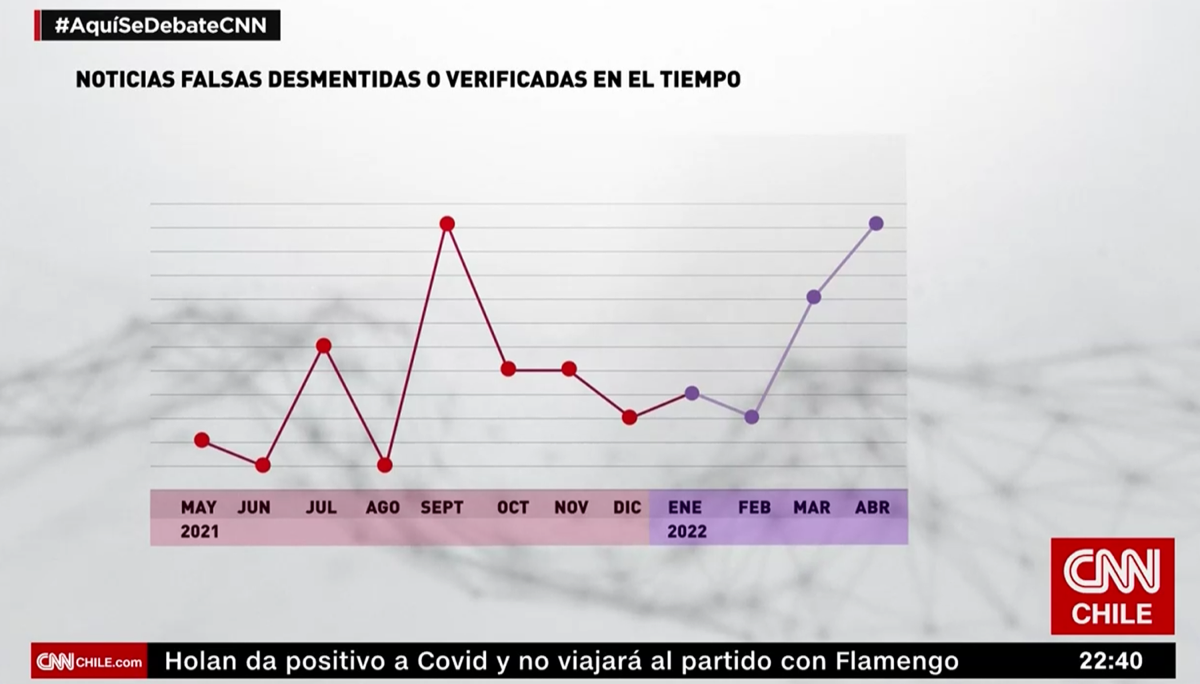
\includegraphics[width=0.32\linewidth]{imagenes/nf_en_tiempo_plesbicito_opt.png}}
    \hfill
    \fcolorbox{uclight}{white}{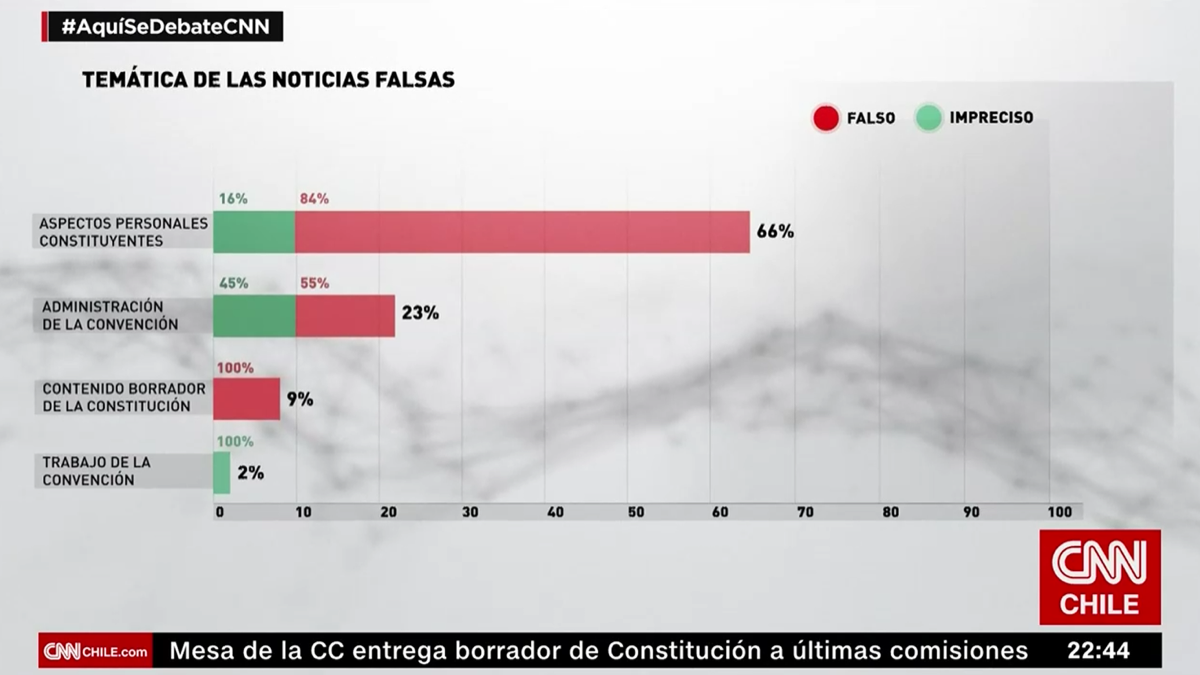
\includegraphics[width=0.32\linewidth]{imagenes/tematicas_nf_plesbicito_opt.png}}
    
    {\fontsize{12}{15}\selectfont \textit{Fuente: Plataforma Telar (M. Salda\~na, PUC)}}
\end{center}

\vspace{0.2cm}

\subsection*{\textcolor{ucred}{\textbf{2024-2025: Red de Bots AFP}}}
\begin{center}
\begin{tikzpicture}[node distance=1.0cm, auto, >=stealth, thick, scale=0.72, transform shape]
    \node[draw, rectangle, fill=ucblue, text=white, font=\bfseries, drop shadow] (afp) {ASOCIACIÓN AFP};
    \node[draw, rectangle, fill=uclight, below=of afp, align=center] (ciudadanos) {Ciudadanos en Acción\\(Bernardo Fontaine)};
    \node[draw, rectangle, fill=ucred, text=white, below left=of ciudadanos, xshift=-0.5cm] (bots) {BOTS/TROLLS};
    \node[draw, rectangle, fill=ucred, text=white, below right=of ciudadanos, xshift=0.5cm] (influ) {INFLUENCERS};
    \node[draw, ellipse, fill=darktext, text=white, below=of ciudadanos, yshift=-1.5cm, drop shadow] (fake) {DESINFORMACIÓN};

    \draw[->, line width=2pt] (afp) -- node[right, font=\small] {Financiamiento Secreto} (ciudadanos);
    \draw[->, line width=2pt] (ciudadanos) -- (bots);
    \draw[->, line width=2pt] (ciudadanos) -- (influ);
    \draw[->, line width=2pt] (bots) -- (fake);
    \draw[->, line width=2pt] (influ) -- (fake);

    % Source
    \node[below=0.2cm of fake, font=\scriptsize\itshape, text=gray] {Fuente: Investigación CIPER / Denuncia G. Winter};
\end{tikzpicture}
\end{center}

\subsection*{\textbf{\textcolor{darktext}{La Estrategia del Miedo (4 Pilares)}}}
{\fontsize{20}{24}\selectfont
Herramienta narrativa para paralizar o movilizar mediante pánico:
\begin{enumerate}
    \setlength{\itemsep}{0.15cm}
    \item \textbf{Ahorros}: Miedo a pérdida de fondos propios.
    \item \textbf{Vivienda}: Miedo a expropiación.
    \item \textbf{Salud}: Miedo al colapso del sistema.
    \item \textbf{Educación}: Miedo a desaparición de escuelas.
\end{enumerate}
}
{\fontsize{20}{24}\selectfont
\textbf{Arquitectura:} Financiamiento opaco de AFP triangulado vía agencia Artool para proteger el modelo.

\textbf{Operación:} Liderada por Bernardo Fontaine (Comando Kast) para atacar reformas y candidatas (Matthei/Jara).

\textbf{Táctica:} ``Infantería digital'' automatizada para instalar narrativas de miedo (expropiación) y desprestigio personal.
}

\end{sectionbox}

% (La sección de referencias reducida aparece a continuación)
\begin{sectionbox}{ucgreen}{REFERENCIAS}
{\fontsize{12}{14}\selectfont
    \begin{center}
        \begin{minipage}{0.24\linewidth}\centering
            \begin{minipage}[c]{0.86\linewidth}\centering
                
\includegraphics[width=0.9\linewidth]{imagenes/frame.png}
            \end{minipage}\hfill
            \begin{minipage}[c]{0.18\linewidth}\centering
                {\fontsize{10}{12}\selectfont \textbf{LINKS EN NOTION}}
            \end{minipage}
        \end{minipage}
        \hfill
        \begin{minipage}{0.24\linewidth}\centering
            \begin{minipage}[c]{0.86\linewidth}\centering
                
\includegraphics[width=0.9\linewidth]{imagenes/frame2.png}
            \end{minipage}\hfill
            \begin{minipage}[c]{0.18\linewidth}\centering
                {\fontsize{10}{12}\selectfont \textbf{PROYECTO EN GITHUB}}
            \end{minipage}
        \end{minipage}
    \end{center}
}
\end{sectionbox}